
\subsection{Benchmark Microservice Systems \& Data Collection}

We deploy three well-known benchmark microservice systems, namely Online Boutique \cite{ob}, Sock Shop \cite{sockshop}, and Train Ticket \cite{tt}, on a Kubernetes cluster consisting of one master node and five worker nodes. Each node has 16 CPUs and 32GB RAM, resulting in a total of 80 CPUs and 160GB RAM across five workers. We sequentially deployed the three systems with their default replicas configuration, i.e., one instance per service, to inject faults and gather metrics data under the load of 100-200 concurrent users. Online Boutique is an e-commerce application with 12 services, allowing users to view items, add them to their cart and make purchases. Each service in the Online Boutique system requires between 0.2-0.5 CPU and 64-512MB RAM for normal functioning. Sock Shop is another e-commerce system focused on selling socks, comprising 11 services that communicate via HTTP requests. Each service in the Sock Shop system requires between 0.1-1 CPU and 300MB-2GB RAM for normal functioning. On the other hand, Train Ticket is one of the largest microservice benchmark systems emulating a train ticket booking platform featuring 64 services. Compared to Sock Shop and Online Boutique, Train Ticket has longer and more complex failure propagation paths. Each service in the Train Ticket system requires between 0.2-1 CPU and 200MB-1GB RAM for normal functioning. These benchmark microservice systems have been widely recognized and employed for evaluating the performance of RCA methods \cite{Jinjin2018Microscope, Azam2022rcd, wu2021microdiag, Xin2023CausalRCA, wu2022automatic, he2022graph, dan2021practical, yu2021microrank, zhou2018trainticket, Wang2021evalcausal}.

\begin{figure}[H]
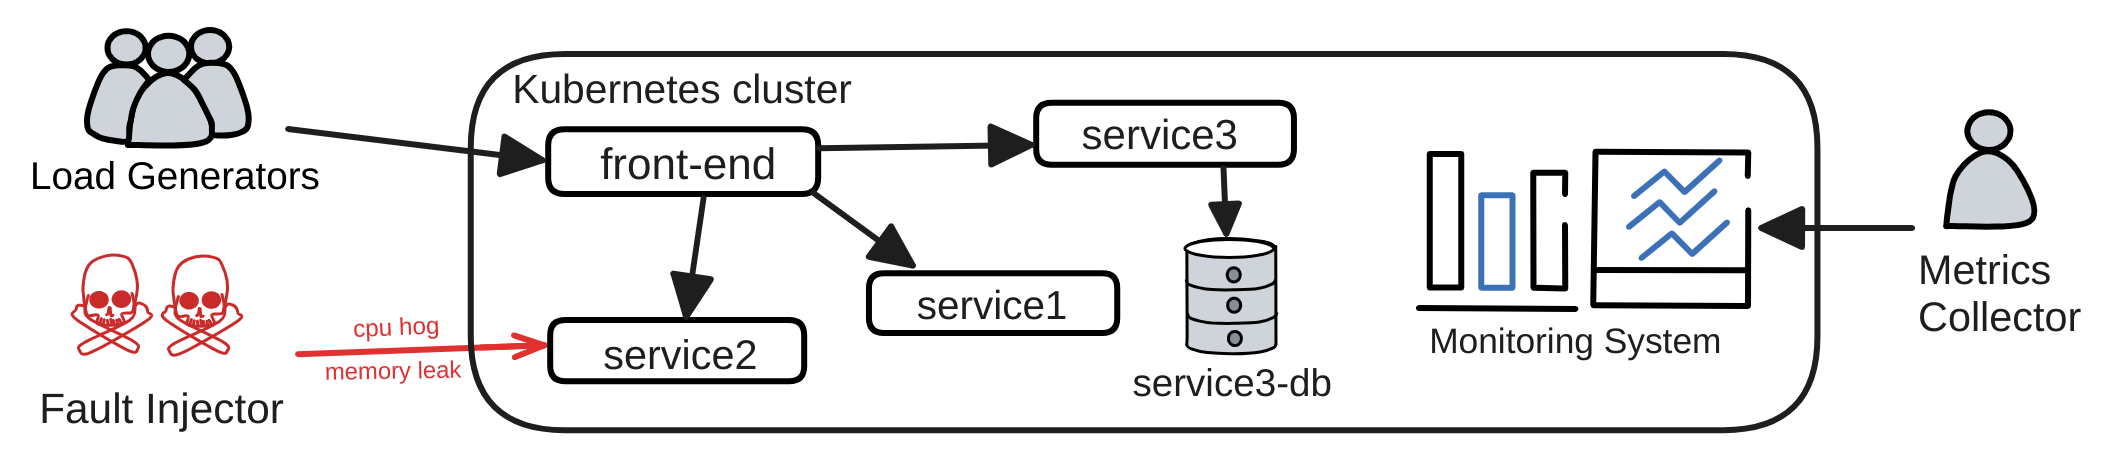
\includegraphics[width=0.8\textwidth]{image/experimental_system_setup_3.png}
\vspace{-0.3cm}
\caption{Overview of our setup for microservice systems.} \label{fig:system_setup}
\vspace{-0.3cm}
\end{figure}

To gather the metrics data, we employ the Istio service mesh \cite{istio} along with Prometheus \cite{prometheus} and cAdvisor \cite{cadvisor} to monitor and collect resource-level and service-level metrics, as previously done in~\cite{Azam2022rcd, Xin2023CausalRCA, wu2021microdiag}. To generate traffic, we use the load generators supplied by these systems and tailor them to explore all services with the load of 40-50 requests per second. Fig. \ref{fig:system_setup} illustrates our setup to collect the experimental data from the microservice systems.

We inject four common anomalies: CPU hog, memory leak, network delay, and packet loss into several key services within each benchmark microservice system. Initially, we operate the applications normally %for 10 minutes 
to gather metrics data under normal conditions. Then, we follow the existing practice \cite{Azam2022rcd, lee2023eadro, wu2021microdiag, Xin2023CausalRCA, yu2021microrank} to inject faults into the running services. We execute into the designated container using kubectl exec. For CPU hog and memory leak, we use stress-ng \cite{stressng} to stress the container resource. For network delay and packet loss, we use tc \cite{tc} to manipulate the traffic of the container. Specifically, we inject faults into five targeted services of Sock Shop (carts, catalogue, orders, payment, and user), five targeted services of Online Boutique (adservice, cartservice, checkoutservice, currencyservice, and productcatalogue), and five targeted services of Train Ticket (ts-auth-service, ts-order-service, ts-route-service, ts-train-service, ts-travel-service). We choose these services due to their critical nature, as issues with their performance can impact other services~\cite{Azam2022rcd, Xin2023CausalRCA, lee2023eadro}. For each combination of fault type and targeted service, we repeat the operation (i.e. fault injection and metrics data collection) five times, resulting in 100 failure cases for each benchmark microservice system. 

Furthermore, to ensure the independence of different injection experiments, we chose to restart the microservice systems after each experiment of injecting failures and collecting data, instead of waiting for a cooldown period, as described in previous studies \cite{wu2021microdiag, yu2021microrank, Xin2023CausalRCA}. Upon visual inspections, we observed that the deviations between the fault injection time and the onset of failure symptoms in the metrics data are usually around 1-3 seconds. 
It is important to note that we simulate a workload of 100-200 concurrent users to interact with the systems intensively. Henceforth, the system is highly sensitive to the injected faults, and anomalies are reflected in the metrics shortly after the injection operation. Table \ref{tab:real-data} presents the statistics summarizing the collected data. To the best of our knowledge, we are the first to use all three popular benchmark microservice systems to evaluate the RCA methods. 

\begin{table}
\centering
\caption{Characteristics of collected data from three benchmark microservice systems (\#metrics, \#svc, \#t\_svc: number of metrics, services, and targeted services in the system. \#fault: number of fault types).} \label{tab:real-data}
\vspace{-0.2cm}
\resizebox{0.6\textwidth}{!}{%
\begin{tabular}{l r r r r r r}
\hline
\textbf{Name} & \textbf{\#metrics}  & \textbf{\#svc}   & \textbf{\#t\_svc}  & \textbf{\#fault} & \textbf{\#cases} \\ \hline \hline
Online Boutique & 49 & 12 & 5  & 4 & 100  \\ \hline
Sock Shop & 46 & 11 & 5 & 4 & 100   \\ \hline
Train Ticket & 212 & 64 & 5 & 4 & 100  \\ \hline
\end{tabular}%
}

\end{table}



\subsection{Evaluation Metrics}


\subsubsection{Anomaly Detection}
Similar to previous works \cite{Chen2014Causeinfer, chen2016causeinfer, chen2022adaptive}, we evaluate the anomaly detectors as binary classification models as the main goal is to detect whether there exist anomalies in the metrics data. We determine metrics data collected during a fault injection period as abnormal, while metrics data before that period is considered normal. Therefore, we use Precision, Recall, and F1 scores to evaluate the anomaly detectors. When an anomaly detection algorithm successfully detects an abnormal sample (i.e., a case with anomalies), it is counted as a True Positive (TP). Conversely, incorrectly classifying an abnormal sample as normal is considered False Negative (FN). Likewise, incorrectly classifying a normal sample as abnormal is considered False Positive (FP). The formulas for computing the metrics Precision, Recall, and F1-score are as follows:
\begin{equation}
    Precision = \frac{TP}{TP + FP}, \quad Recall = \frac{TP}{TP + FN}, \quad F1 = \frac{2\times Precision \times Recall}{Precision + Recall}.
\end{equation}


\subsubsection{Root Cause Analysis}

Following existing works \cite{Wang2018cloudranger, Ma2019Msrank, Ma2020Automap, Meng2020Microcause, yu2021microrank, wu2020microrca, wu2021microdiag, Azam2022rcd, Li2022Circa, Xin2023CausalRCA}, we use two standard metrics, namely $AC@k$ and $Avg@k$ to assess the performance of the RCA methods. Herein, we set $k = 1, 3, 5$. Given a set of failure cases A, $AC@k$ and $Avg@k$ are calculated as follows,
\begin{equation}
    AC@k = \frac{1}{|A|} \sum\nolimits_{a\in A}\frac{\sum_{i<k}R^a[i]\in V^a_{rc}}{min(k, |V^a_{rc}|)}, \quad Avg@k = \frac{1}{k}\sum_{j=1}^k AC@j.
\end{equation}
where $R^a[i]$ denotes the $i$th ranking result for the failure case $a$ by an RCA method, and $V^a_{rc}$ is the true root cause set of case $a$. $AC@k$ represents the probability the top $k$ results given by a method include the real root causes. It ranges from $0$ to $1$, with higher values indicating better performance.
Meanwhile, $Avg@k$ measures the overall performance of RCA methods.

% Following existing works \cite{Wang2018cloudranger, Ma2019Msrank, Ma2020Automap, Meng2020Microcause, yu2021microrank, wu2020microrca, wu2021microdiag, Azam2022rcd, Li2022Circa, Xin2023CausalRCA}, we use two standard metrics, namely $AC@k$ and $Avg@k$ to assess the performance of the RCA methods. Herein, we set $k = 1, 3, 5$. Given a set of failure cases A, $AC@k$ is calculated as follows,
% \begin{equation}
%     AC@k = \frac{1}{|A|} \sum\nolimits_{a\in A}\frac{\sum_{i<k}R^a[i]\in V^a_{rc}}{min(k, |V^a_{rc}|)},
% \end{equation}
% where $R^a[i]$ denotes the $i$th ranking result for the failure case $a$ by an RCA method, and $V^a_{rc}$ is the true root cause set of case $a$. $AC@k$ represents the probability the top $k$ results given by a method include the real root causes. It ranges from $0$ to $1$, with higher values indicating better performance.
% $Avg@k$, which measures the overall performance of RCA methods, is calculated as follows,
% \begin{equation}
%     Avg@k = \frac{1}{k}\sum_{j=1}^k AC@j.
% \end{equation}


\subsection{Experimental Setting}
We conduct all the experiments on Linux servers equipped with 8 CPU and 16GB RAM. To avoid any randomness, when evaluating each method, for each failure case we repeat the experiment (detecting anomalies and identifying root causes) five times, then report the average results. Our framework is implemented using Python 3.10.


\vspace{-0.2cm}
\subsection{Baselines} \label{sec:baselines}

\paragraph{Anomaly Detection Baselines.} We select the following four baselines to compare against our proposed method: \textit{N-Sigma} \cite{Jinjin2018Microscope, Li2022Circa}, \textit{BIRCH} \cite{zhang1996birch, wu2020microrca, wu2021microdiag}, \textit{SPOT} \cite{siffer2017anomaly, pan2021dycauserca, Li2022Circa, lee2023eadro, Meng2020Microcause}, and \textit{Univariate Bayesian Change Point Detection} (denoted as UniBCP) \cite{adams2007bayesian, Chen2014Causeinfer, chen2016causeinfer}. These methods are commonly used in existing RCA research for anomaly detection. Their source code has been made publicly available, with the exception of UniBCP, for which we leverage an available implementation \cite{unibcp} for the evaluation. The detailed descriptions of these methods are in Section \ref{sec:background-ad}. For all methods, we use the hyperparameter settings as in previous works and in their public source code. 


\vspace{-0.2cm}
\paragraph{Root Cause Analysis Baselines.} We choose six representative baselines, including five state-of-the-art metric-based RCA methods: CausalRCA \cite{Xin2023CausalRCA}, RCD \cite{Azam2022rcd}, CIRCA \cite{Li2022Circa}, $\epsilon$-Diagnosis \cite{Shan2019Ediagnosis}, and N-Sigma \cite{Li2022Circa}, for performance comparison with our proposed method, BARO. Detailed information of these methods is as follows:

\begin{itemize}
\item \textit{Dummy:} Dummy randomly selects a metric as the root cause. We use this method to assess whether our BARO framework and the other baselines outperform random selection.

\item \textit{CausalRCA \cite{Xin2023CausalRCA}:} CausalRCA uses DAG-GNN \cite{Yu2019DagGNN}, a gradient-based causal structure learning method, to estimate the causal graph and uses PageRank algorithm to rank the root causes.

\item \textit{$\epsilon$-Diagnosis \cite{Shan2019Ediagnosis}:}
 $\epsilon$-Diagnosis uses the two-sample test algorithm and $\epsilon$-statistics to estimate the similarity between every pair of metrics and rank the root causes based on test scores. 
 

\item \textit{RCD \cite{Azam2022rcd}:} RCD employs a divide-and-conquer strategy to divide the input metrics into smaller chunks. It uses the $\Psi$-PC algorithm \cite{Jaber2020PsiFCI} to construct a causal graph and identify root causes within each chunk. Subsequently, it combines these root causes and repeats this process until only one chunk remains.


\item \textit{CIRCA \cite{Li2022Circa}:} CIRCA creates a causal graph by using a provided call graph, which requires operational knowledge. Then, it performs regression-based hypothesis testing to find the root causes. Since the call graph is not available, thus following \cite{Azam2022rcd, liu2023pyrca}, we use the PC algorithm to construct this graph for CIRCA. 

\item \textit{N-Sigma \cite{Jinjin2018Microscope,Li2022Circa}:} N-Sigma is a statistical analysis technique that compares the metrics data before and after the anomaly detection time using z-score. The higher the score, the more likely that metric is the root cause of the failure. 

\end{itemize}

The source code of CausalRCA, RCD, CIRCA, and N-Sigma is publicly available. For CIRCA, since the required call graphs are unavailable, we use the PC algorithm to construct the causal graphs as done in \cite{Azam2022rcd, Ma2019Msrank, Ma2020Automap, Wang2018cloudranger, Xin2023CausalRCA}. For $\epsilon$-Diagnosis, the original source code is unavailable thus we rely on the implementation of a related work \cite{liu2023pyrca}. We use the same hyperparameter values as reported in their papers.




\subsection{RQ1: Effectiveness in Anomaly Detection}


In this RQ, we evaluate the performance of BARO and the baseline anomaly detectors across all three datasets. We use the metrics data collected before the failure as normal data, and during the failure as abnormal data. We report the average of Precision (Pre), Recall (Rec), and F1-score (F1) over all the cases. Table \ref{tab:ad1} presents the experimental results, with the best results highlighted in \textbf{bold}. We draw the following observations:

\textbf{(1) BARO consistently outperforms all baseline methods in detecting anomalies by a large margin across all three benchmark microservice systems.} It achieves the highest Precision, Recall, and F1-score on all the datasets. BARO's performance can be attributed to the following factors: (1) BOCPD's ability to detect distribution changes, suitable for identifying anomalies from the failure, acting as a soft intervention \cite{Azam2022rcd, Li2022Circa}, (2) Multivariate BOCPD considers not only individual time series but also the dependencies among the time series, allowing it to detect correlation changes, and (3) it does not require any user-defined thresholds making it to be highly adaptive to different types of metrics data.


\begin{table}
\centering
\caption{Precision, Recall, and F1-score of five anomaly detectors on three datasets: Online Boutique, Sock Shop, and Train Ticket. The best scores are in \textbf{bold}. Higher values indicate better performance.}
\vspace{-0.2cm}
\label{tab:ad1}
\resizebox{0.68\textwidth}{!}{%
\begin{tabular}{l|rrr|rrr|rrr}
\hline
 & \multicolumn{3}{c|}{\textbf{Online Boutique}} & \multicolumn{3}{c|}{\textbf{Sock Shop}} & \multicolumn{3}{c}{\textbf{Train Ticket}} \\ \cline{2-10} 
Method & \multicolumn{1}{c}{\textit{Pre}} & \multicolumn{1}{c}{\textit{Rec}} & \multicolumn{1}{c|}{\textit{F1}} & \multicolumn{1}{c}{\textit{Pre}} & \multicolumn{1}{c}{\textit{Rec}} & \multicolumn{1}{c|}{\textit{F1}} & \multicolumn{1}{l}{\textit{Pre}} & \multicolumn{1}{l}{\textit{Rec}} & \multicolumn{1}{c}{\textit{F1}}  \\ \hline
N-Sigma & 0.54 & \textbf{1} & 0.7 & 0.56 & \textbf{1} & 0.72 & 0.5 & 1 & 0.67 \\ \hline
SPOT & 0.53 & \textbf{1} & 0.69 & 0.53 & \textbf{1} & 0.69 & 0.5 & 1 & 0.67 \\ \hline
BIRCH & 0.35 & 0.48 & 0.4 & 0.05 & 0.05 & 0.05 & 0.39 & 0.4 & 0.39 \\ \hline
UniBCP & 0.51 & \textbf{1} & 0.67 & 0.5 & 0.99 & 0.66 & 0.5 & 1 & 0.67 \\ \hline
\textbf{BARO (Ours)} & \textbf{0.69} & \textbf{1} & \textbf{0.82} & \textbf{0.6} & \textbf{1} & \textbf{0.75} & \textbf{0.68} & \textbf{1} & \textbf{0.81} \\ \hline
\end{tabular}%
}

{\footnotesize \textit{(*) UniBCP denotes Univariate Offline Bayesian Change Point Detection.}}

\vspace{-0.2cm}
\end{table}


\textbf{(2) All baseline methods, except BIRCH, have very high recalls but low precisions across all the datasets.} This indicates that they generally can detect anomalies, however, they also frequently misclassify normal time series as anomalous. The precision of these methods generally range from 0.05 to 0.68. Based on our observations, this is due to the complexity and dynamics of the benchmark microservice systems, which include many time series metrics with complicated patterns, leading to frequent misclassifications of anomalies by these baseline methods.

In summary, BARO stands out as the best-performing method, being effective in detecting anomalies. This anomaly detection capability plays a crucial role in the subsequent RCA task. 


\subsection{RQ2: Effectiveness in Root Cause Analysis}

In this section, we evaluate the performance of BARO and the RCA baseline methods on all three datasets. First, we assess the ideal performance of the methods when the anomaly occurrence time is known accurately. Specifically, we use the fault injection time $t_{\text{inject}}$ as a proxy for the true anomaly occurence time since we have observed that in our benchmark microservice systems, the anomaly occurence time closely aligns with the fault injection time. Then, we assess the performance of RCA methods when using the anomaly detection time provided by existing anomaly detectors described in Section \ref{sec:baselines}. Note that Dummy and CausalRCA do not require the specification of the anomaly detection time. Tables \ref{tab:q2-rca-s} and \ref{tab:q2-rca-f1} report the overall performance of all methods using the Avg@5 scores for coarse-grained root cause analysis (root cause services) and fine-grained root cause analysis (root cause metrics), respectively. We calculate the accuracy for each type of fault: CPU hog (CPU), memory leak (MEM), network delay (DELAY), and packet loss (LOSS), as well as their average (AVG) to report the overall performance across four fault types. In the tables, we denote the combination of an RCA method and an anomaly detector as \textit{RCA\_method[Anomaly\_Detector]}. For instance, RCD[N-Sigma], RCD[BIRCH], RCD[SPOT], RCD[UniBCP], and RCD[BOCPD] represent the RCA pipelines that combine RCD with the anomaly detectors N-Sigma, BIRCH, SPOT, Univariate BCPD, and Multivariate BOCPD, respectively.


\begin{table}[]
\centering
\caption{Coarse-grained performance of different RCA methods in terms of Avg@5 on three different datasets. The fault types CPU, MEM, DELAY, and LOSS denote CPU overload, memory leak, network delay, and packet loss. The highest scores are in \textbf{bold}, and the second highest scores are in {\ul underscore}.}
\label{tab:q2-rca-s}
\vspace{-0.2cm}
\resizebox{\textwidth}{!}{%
\setlength\tabcolsep{3pt}
\begin{tabular}{l|rrrrr|rrrrr|rrrrr}
\hline
 & \multicolumn{5}{c|}{\textbf{Online Boutique}} & \multicolumn{5}{c|}{\textbf{Sock Shop}} & \multicolumn{5}{c}{\textbf{Train Ticket}} \\ \cline{2-16} 
Method & \multicolumn{1}{c}{\textit{CPU}} & \multicolumn{1}{c}{\textit{MEM}} & \multicolumn{1}{c}{\textit{DELAY}} & \multicolumn{1}{c}{\textit{LOSS}} & \multicolumn{1}{c|}{\textit{AVG}} & \multicolumn{1}{c}{\textit{CPU}} & \multicolumn{1}{c}{\textit{MEM}} & \multicolumn{1}{c}{\textit{DELAY}} & \multicolumn{1}{c}{\textit{LOSS}} & \multicolumn{1}{c|}{\textit{AVG}} & \multicolumn{1}{c}{\textit{CPU}} & \multicolumn{1}{c}{\textit{MEM}} & \multicolumn{1}{c}{\textit{DELAY}} & \multicolumn{1}{c}{\textit{LOSS}} & \multicolumn{1}{c}{\textit{AVG}} \\ \hline \hline
Dummy & 0.24 & 0.26 & 0.27 & 0.24 & 0.25 & 0.37 & 0.41 & 0.38 & 0.37 & 0.38 & 0.07 & 0.08 & 0.07 & 0.07 & 0.07 \\
CausalRCA & 0.85 & 0.91 & 0.86 & 0.58 & 0.8 & 0.49 & 0.82 & 0.61 & 0.47 & 0.6 & 0.53 & 0.3 & 0.17 & 0.11 & 0.28 \\ \hline
$\epsilon$-Diagnosis {[}$t_{\text{inject}}${]} & 0.1 & 0.13 & 0.12 & 0.12 & 0.12 & 0.47 & 0.3 & 0.42 & 0.49 & 0.42 & 0 & 0.02 & 0 & 0 & 0.01 \\
$\epsilon$-Diagnosis {[}N-Sigma{]} & 0.19 & 0.16 & 0.23 & 0.22 & 0.2 & 0.49 & 0.39 & 0.46 & 0.5 & 0.46 & 0 & 0 & 0 & 0.02 & 0.01 \\
$\epsilon$-Diagnosis {[}BIRCH{]} & 0.23 & 0.33 & 0.21 & 0.14 & 0.22 & - & 0 & - & 1 & 0.8 & 0.07 & 0 & 0 & 0 & 0.02 \\
$\epsilon$-Diagnosis {[}SPOT{]} & 0.37 & 0.2 & 0.17 & 0.22 & 0.24 & 0.46 & 0.34 & 0.42 & 0.46 & 0.42 & 0 & 0.02 & 0 & 0 & 0.01 \\
$\epsilon$-Diagnosis {[}UniBCP{]} & 0.28 & 0.09 & 0.4 & 0.2 & 0.24 & 0.2 & 0.19 & 0.25 & 0.2 & 0.21 & 0.05 & 0.10 & 0.08 & 0.04 & 0.07  \\
$\epsilon$-Diagnosis {[}BOCPD{]} & 0.23 & 0.09 & 0.18 & 0.15 & 0.16 & 0.45 & 0.35 & 0.38 & 0.44 & 0.41 & 0 & 0 & 0 & 0.06 & 0.02 \\ \hline
RCD {[}$t_{\text{inject}}${]} & 0.69 & 0.4 & 0.27 & 0.5 & 0.47 & 0.62 & 0.46 & 0.48 & 0.37 & 0.48 & 0.08 & 0.01 & 0.09 & 0.12 & 0.08 \\
RCD {[}N-Sigma{]} & 0.67 & 0.43 & 0.31 & 0.49 & 0.48 & 0.54 & 0.42 & 0.46 & 0.37 & 0.45 & 0.07 & 0 & 0.05 & 0.1 & 0.06 \\
RCD {[}BIRCH{]} & 0.69 & 0.37 & 0.28 & 0.50 & 0.46 & 0.57 & 0.42 & 0.49 & 0.37 & 0.46 & 0.06 & 0 & 0.03 & 0.11 & 0.05 \\
RCD {[}SPOT{]} & 0.7 & 0.42 & 0.3 & 0.48 & 0.48 & 0.58 & 0.43 & 0.46 & 0.34 & 0.45 & 0.08 & 0.01 & 0.07 & 0.09 & 0.06 \\
RCD {[}UniBCP{]} & 0.66 & 0.42 & 0.29 & 0.49 & 0.47 & 0.62 & 0.44 & 0.5 & 0.36 & 0.48 & 0.05 & 0.01 & 0.05 & 0.1 & 0.05 \\
RCD {[}BOCPD{]} & 0.7 & 0.4 & 0.3 & 0.52 & 0.48 & 0.6 & 0.47 & 0.48 & 0.36 & 0.48 & 0.06 & 0 & 0.04 & 0.09 & 0.05 \\ \hline
CIRCA {[}$t_{\text{inject}}${]} & {\ul 0.9} & 0.74 & 0.9 & 0.55 & 0.77 & {\ul 0.97} & \textbf{0.98} & {\ul 0.98} & {\ul 0.88} & {\ul 0.95} & 0.66 & 0.93 & 0.64 & 0.57 & 0.7 \\
CIRCA {[}N-Sigma{]} & 0.78 & 0.59 & 0.79 & 0.48 & 0.66 & 0.86 & 0.7 & 0.87 & 0.7 & 0.78 & 0.65 & 0.88 & 0.58 & 0.57 & 0.67 \\
CIRCA {[}BIRCH{]} & 0.45 & 0.38 & 0.27 & 0.48 & 0.39 & - & 0.60 & - & 0.75 & 0.72 & 0.10 & 0 & 0.35 & 0.13 & 0.19 \\
CIRCA {[}SPOT{]} & 0.76 & 0.7 & 0.88 & 0.66 & 0.75 & 0.83 & 0.87 & 0.95 & 0.78 & 0.86 & 0.69 & 0.96 & 0.58 & 0.53 & 0.69 \\
CIRCA {[}UniBCP{]} & 0.16 & 0 & 0 & 0.35 & 0.13 & 0.23 & 0 & 0.2 & 0.36 & 0.2 & 0 & 0 & 0 & 0.33 & 0.08 \\
CIRCA {[}BOCPD{]} & 0.68 & 0.2 & 0.28 & 0.42 & 0.4 & 0.73 & \textbf{0.98} & 0.54 & 0.66 & 0.73 & 0.37 & 0.12 & 0.3 & 0.17 & 0.24 \\ \hline
N-Sigma {[}$t_{\text{inject}}${]} & {\ul 0.9} & 0.93 & {\ul 0.94} & 0.66 & \textbf{0.86} & \textbf{0.98} & \textbf{0.98} & {\ul 0.98} & \textbf{0.9} & \textbf{0.96} & 0.81 & 0.96 & 0.61 & \textbf{0.7} & 0.77 \\
N-Sigma {[}N-Sigma{]} & 0.79 & 0.69 & 0.83 & 0.63 & 0.74 & 0.85 & 0.77 & 0.89 & 0.79 & 0.83 & 0.74 & \textbf{0.98} & 0.61 & 0.65 & 0.75 \\
N-Sigma {[}BIRCH{]} & 0.83 & 0.78 & 0.64 & 0.6 & 0.71 & 		
- & 0 & - & 0.85 & 0.68 & 0.55 & 0.7 & 0.47 & 0.45 & 0.51 \\
N-Sigma {[}SPOT{]} & 0.79 & 0.79 & 0.93 & 0.65 & 0.79 & 0.87 & 0.91 & \textbf{0.99} & 0.82 & 0.9 & 0.75 & \textbf{0.98} & 0.61 & 0.64 & 0.75 \\
N-Sigma {[}UniBCP{]} & 0.75 & 0.69 & 0.91 & {\ul 0.76} & 0.78 & 0.86 & 0.79 & 0.69 & 0.81 & 0.79 & 0.38 & 0.71 & 0.38 & 0.62 & 0.52 \\
N-Sigma {[}BOCPD{]} & 0.74 & 0.32 & 0.52 & 0.58 & 0.54 & 0.8 & \textbf{0.98} & 0.63 & 0.62 & 0.76 & 0.51 & 0.16 & 0.29 & 0.22 & 0.3 \\ \hline 
RobustScorer {[}$t_{\text{inject}}${]} & {\ul 0.9} & {\ul 0.94} & {\ul 0.94} & 0.65 & \textbf{0.86} & \textbf{0.98} & \textbf{0.98} & {\ul 0.98} & 0.86 & {\ul 0.95} & \textbf{0.9} & {\ul 0.97} & {\ul 0.62} & {\ul 0.67} & {\ul 0.79} \\
RobustScorer {[}N-Sigma{]} & {\ul 0.9} & \textbf{0.96} & 0.88 & 0.58 & 0.83 & 0.96 & \textbf{0.98} & {\ul 0.98} & \textbf{0.9} & \textbf{0.96} & 0.82 & \textbf{0.98} & {\ul 0.62} & 0.64 & 0.77 \\
RobustScorer {[}BIRCH{]} & 0.92 & 0.93 & 0.81 & 0.51 & 0.79 & - & 1 & - & 0.85 & 0.88 & 0.76 & 0.55 & 0.57 & 0.71 & 0.65 \\
RobustScorer {[}SPOT{]} & 0.89 & {\ul 0.94} & 0.93 & 0.61 & {\ul 0.84} & {\ul 0.97} & \textbf{0.98} & \textbf{0.99} & 0.86 & {\ul 0.95} & {\ul 0.85} & \textbf{0.98} & 0.61 & 0.66 & 0.78 \\
RobustScorer {[}UniBCP{]} & 0.73 & 0.67 & 0.89 & \textbf{0.79} & 0.77 & 0.8 & 0.65 & 0.69 & 0.84 & 0.75 & 0.37 & 0.64 & 0.38 & 0.54 & 0.48 \\ \hline
\textbf{BARO (Ours)} & \textbf{0.91} & \textbf{0.96} & \textbf{0.95} & 0.62 & \textbf{0.86} & {\ul 0.97} & \textbf{0.98} & {\ul 0.98} & 0.87 & {\ul 0.95} & \textbf{0.9} & \textbf{0.98} & \textbf{0.64} & \textbf{0.7} & \textbf{0.81} \\ \hline
\end{tabular}%
}

{\footnotesize \textit{(*) BIRCH has a poor recall, so RCA results with BIRCH are obtained from a limited number of failure cases where BIRCH detects anomalies.
CIRCA results for TrainTicket are only obtained from 15/100 cases due to PC's failed causal graph construction.
}}
\vspace{-0.3cm}
\end{table}

% (*) BIRCH has a poor recall, so the results of RCA methods combined with BIRCH are calculated based on a limited number of failure cases.
% CIRCA results for Train Ticket are only obtained from 15/100 cases due to PC's failed causal graph construction.


\subsubsection{Coarse-grained Root Cause Analysis}

From Table \ref{tab:q2-rca-s}, we draw the following observations.

\textbf{(1) BARO performs the best in identifying the coarse-grained root cause of the failure}, consistently achieving top accuracy scores for all types of faults across all datasets. BARO achieves the highest Avg@5 in 10 out of 15 cases and outperforms other baselines by a large margin. For example, while CausalRCA achieves 0.8, 0.6, and 0.28, BARO achieves 0.86, 0.95, and 0.81 in the overall Avg@5 for all three microservice systems, respectively. This represents 7.5\%, 58\%, and 189\% improvements compared to CausalRCA.



From the results, we can see that, when working with large-scale microservice systems, $\epsilon$-Diagnosis, RCD, CausalRCA, and CIRCA encounter huge difficulties, whereas BARO yields much better results. BARO's resistance to the imprecision of the anomaly detection time via the nonparametric RobustScorer hypothesis test demonstrates its applicability in practical scenarios, where the anomaly detection module may differ across real-world systems. Moreover, BARO leverages multivariate BOCPD to capture dependencies within multivariate metrics data, allowing for more precise localization of the anomaly occurrence time and thus improve the RCA performance. 


\textbf{(2) CausalRCA does not require separating the normal and abnormal metrics data.} It uses all the provided metrics data to construct the causal graph and then uses PageRank to rank the root causes. The experimental results indicate that it performs well on the Online Boutique system. For instance, it achieves an Avg@5 of 0.85 for the CPU overload fault, 0.91 for the memory leak fault, and an overall Avg@5 of 0.8. Nevertheless, its performance declines on the other two systems. For example, it only achieves overall Avg@5 scores of 0.6 and 0.28 on the Sock Shop and Train Ticket systems, possibly due to the challenges posed by the complex structures of these systems. Overall, we can see that the performance of CausalRCA varies significantly across different systems.

\textbf{(3) $\epsilon$-Diagnosis, a widely-known baseline RCA method, does not perform greatly superior to random selection.} For example, its overall Avg@5 scores range from 0.12 to 0.24, whereas random selection achieves 0.25 on the Online Boutique system. However, it outperforms Dummy by 20\% in the Sock Shop system, with an overall Avg@5 score of 0.46 compared to Dummy's 0.38.

\textbf{(4) RCD outperforms random selection in small-scale systems such as Online Boutique and Sock Shop.} For example, its overall Avg@5 scores range from 0.45 to 0.48 while Dummy's scores range from 0.25 to 0.38. However, for the large-scale Train Ticket system, RCD's performance drops remarkably. For instance, RCD's Avg@5 scores range from 0.05 to 0.08, similar to Dummy's. This observation suggests the need to include large-scale systems like Train Ticket in future work to benchmark newly proposed RCA methods.

\textbf{(5) We observe that N-Sigma, a simple statistical analysis technique, performs better than CIRCA.} Note that, in this work, as discussed, for CIRCA, we use the causal graphs constructed by the PC algorithm instead of the required call graphs as these graphs are not available for these systems, which could be a cause of this observation. Overall, N-Sigma outperforms both CIRCA and RCD in coarse-grained root cause localization.

In summary, BARO consistently outperforms other methods for all fault types and datasets by a large margin. When applied to a large-scale system like Train Ticket, baseline methods like $\epsilon$-Diagnosis, RCD, CausalRCA, and CIRCA struggle, while BARO still delivers superior results.


\begin{table}[!t]
\centering
\caption{Fine-grained performance of different RCA methods in terms of Avg@5 accuracy on three different datasets. The fault types CPU, MEM, DELAY, and LOSS denote CPU overload, memory leak, network delay, and packet loss. The highest scores are in \textbf{bold}, and the second highest scores are in {\ul underscore}.}
\label{tab:q2-rca-f1}
\vspace{-0.2cm}
\resizebox{\textwidth}{!}{%
\setlength\tabcolsep{3pt}
\begin{tabular}{l|rrrrr|rrrrr|rrrrr}
\hline
 & \multicolumn{5}{c|}{\textbf{Online Boutique}} & \multicolumn{5}{c|}{\textbf{Sock Shop}} & \multicolumn{5}{c}{\textbf{Train Ticket}} \\ \cline{2-16} 
Method & \multicolumn{1}{c}{\textit{CPU}} & \multicolumn{1}{c}{\textit{MEM}} & \multicolumn{1}{c}{\textit{DELAY}} & \multicolumn{1}{c}{\textit{LOSS}} & \multicolumn{1}{c|}{\textit{AVG}} & \multicolumn{1}{c}{\textit{CPU}} & \multicolumn{1}{c}{\textit{MEM}} & \multicolumn{1}{c}{\textit{DELAY}} & \multicolumn{1}{c}{\textit{LOSS}} & \multicolumn{1}{c|}{\textit{AVG}} & \multicolumn{1}{c}{\textit{CPU}} & \multicolumn{1}{c}{\textit{MEM}} & \multicolumn{1}{c}{\textit{DELAY}} & \multicolumn{1}{c}{\textit{LOSS}} & \multicolumn{1}{c}{\textit{AVG}} \\ \hline \hline
Dummy & 0.08 & 0.06 & 0.07 & 0.06 & 0.07 & 0.1 & 0.07 & 0.07 & 0.06 & 0.08 & 0.02 & 0.02 & 0.02 & 0.01 & 0.02 \\
CausalRCA & \textbf{0.55} & \textbf{0.78} & 0.86 & 0.39 & \textbf{0.65} & 0.39 & 0.42 & 0.49 & 0.34 & 0.41 & 0.51 & 0.13 & 0.1 & 0.09 & 0.21 \\ \hline
$\epsilon$-Diagnosis {[}$t_{\text{inject}}${]} & 0.07 & 0.03 & 0.06 & 0.02 & 0.05 & 0 & 0 & 0 & 0 & 0 & 0 & 0 & 0 & 0 & 0 \\
$\epsilon$-Diagnosis {[}N-Sigma{]} & 0 & 0.06 & 0.2 & 0.13 & 0.1 & 0.02 & 0 & 0 & 0 & 0.01 & 0 & 0 & 0 & 0 & 0 \\
$\epsilon$-Diagnosis {[}BIRCH{]} & 0 & 0.07 & 0.21 & 0.14 & 0.11 &  - & 0 & - & 0 & 0 & 0 & 0 & 0.2 & 0 & 0 \\
$\epsilon$-Diagnosis {[}SPOT{]} & 0.06 & 0.02 & 0.14 & 0.06 & 0.07 & 0 & 0 & 0 & 0 & 0 & 0 & 0 & 0 & 0 & 0 \\
$\epsilon$-Diagnosis {[}UniBCP{]} & 0 & 0 & 0.3 & 0.12 & 0.11 & 0 & 0 & 0.11 & 0.09 & 0.05 & 0.05 & 0 & 0.05 & 0 & 0.03 \\
$\epsilon$-Diagnosis {[}BOCPD{]} & 0.02 & 0.04 & 0.1 & 0.12 & 0.07 & 0 & 0 & 0 & 0 & 0 & 0 & 0 & 0 & 0 & 0 \\ \hline
RCD {[}$t_{\text{inject}}${]} & 0.16 & 0.26 & 0.22 & 0.18 & 0.21 & 0.02 & 0.17 & 0.1 & 0.07 & 0.09 & 0 & 0 & 0.06 & 0 & 0.02 \\
RCD {[}N-Sigma{]} & 0.16 & 0.29 & 0.23 & 0.15 & 0.21 & 0 & 0.16 & 0.09 & 0.07 & 0.08 & 0 & 0 & 0.03 & 0 & 0.01 \\
RCD {[}BIRCH{]} & 0.15 & 0.27 & 0.24 & 0.19 & 0.21 & 0.01 & 0.15 & 0.11 & 0.06 & 0.08 & 0 & 0 & 0.02 & 0 & 0 \\
RCD {[}SPOT{]} & 0.14 & 0.31 & 0.23 & 0.15 & 0.21 & 0.02 & 0.16 & 0.11 & 0.06 & 0.09 & 0 & 0 & 0.04 & 0 & 0.01 \\
RCD {[}UniBCP{]} & 0.16 & 0.31 & 0.22 & 0.14 & 0.21 & 0.01 & 0.16 & 0.09 & 0.07 & 0.08 & 0 & 0 & 0.04 & 0 & 0.01 \\
RCD {[}BOCPD{]} & 0.17 & 0.28 & 0.24 & 0.17 & 0.22 & 0.04 & 0.16 & 0.14 & 0.07 & 0.1 & 0 & 0 & 0.03 & 0 & 0.01 \\ \hline
CIRCA {[}$t_{\text{inject}}${]} & 0.42 & 0.3 & 0.9 & {\ul 0.54} & 0.54 & 0.52 & 0.58 & {\ul 0.98} & {\ul 0.86} & 0.74 & 0.48 & 0.86 & 0.55 & 0.57 & 0.62 \\
CIRCA {[}N-Sigma{]} & 0.22 & 0.27 & 0.79 & 0.4 & 0.42 & 0.5 & 0.42 & 0.87 & 0.66 & 0.61 & 0.48 & 0.84 & 0.51 & 0.54 & 0.59 \\
CIRCA {[}BIRCH{]} & 0.17 & 0 & 0.29 & 0.38 & 0.23 & - & 0 & - & 0.75 & 0.60 & 0.10 & 0 & 0.31 & 0.13 & 0.18 \\
CIRCA {[}SPOT{]} & 0.34 & 0.18 & 0.88 & 0.6 & 0.5 & 0.5 & 0.46 & 0.94 & 0.74 & 0.66 & 0.5 & 0.88 & 0.5 & 0.5 & 0.6 \\
CIRCA {[}UniBCP{]} & 0 & 0 & 0 & 0.2 & 0.05 & 0.08 & 0 & 0 & 0.15 & 0.06 & 0 & 0 & 0 & 0.17 & 0.04 \\
CIRCA {[}BOCPD{]} & 0.29 & 0 & 0.18 & 0.35 & 0.21 & 0.42 & 0.49 & 0.34 & 0.47 & 0.43 & 0.3 & 0.12 & 0.18 & 0.09 & 0.17 \\ \hline
N-Sigma {[}$t_{\text{inject}}${]} & {\ul 0.54} & 0.54 & {\ul 0.94} & 0.5 & {\ul 0.63} & 0.77 & 0.7 & {\ul 0.98} & \textbf{0.88} & {\ul 0.83} & \textbf{0.6} & 0.93 & 0.54 & \textbf{0.65} & \textbf{0.68} \\
N-Sigma {[}N-Sigma{]} & 0.38 & 0.33 & 0.83 & 0.48 & 0.51 & 0.66 & 0.46 & 0.87 & 0.66 & 0.66 & 0.55 & {\ul 0.94} & 0.55 & 0.59 & 0.66 \\
N-Sigma {[}BIRCH{]} & 0.38 & 0.33 & 0.63 & 0.46 & 0.45 & - & 0 & - & 0.85 & 0.68 & 0.33 & 0.65 & 0.39 & 0.33 & 0.38 \\
N-Sigma {[}SPOT{]} & 0.41 & 0.41 & 0.92 & 0.53 & 0.57 & 0.66 & 0.58 & \textbf{0.99} & 0.77 & 0.75 & {\ul 0.56} & {\ul 0.94} & 0.55 & 0.58 & 0.66 \\
N-Sigma {[}UniBCP{]} & 0.37 & 0.11 & 0.91 & 0.66 & 0.51 & 0.51 & 0.08 & 0.59 & 0.74 & 0.48 & 0.2 & 0.39 & 0.38 & {\ul 0.62} & 0.4 \\
N-Sigma {[}BOCPD{]} & 0.46 & 0.04 & 0.51 & 0.46 & 0.37 & 0.6 & 0.54 & 0.42 & 0.52 & 0.52 & 0.35 & 0.16 & 0.21 & 0.14 & 0.22 \\ \hline 
RobustScorer {[}$t_{\text{inject}}${]} & 0.51 & 0.48 & {\ul 0.94} & 0.49 & 0.61 & \textbf{0.81} & 0.68 & {\ul 0.98} & 0.79 & 0.82 & 0.54 & 0.9 & {\ul 0.57} & 0.6 & 0.65 \\
RobustScorer {[}N-Sigma{]} & {\ul 0.54} & {\ul 0.56} & 0.88 & 0.49 & 0.62 & {\ul 0.8} & {\ul 0.72} & {\ul 0.98} & 0.83 & {\ul 0.83} & 0.46 & \textbf{0.96} & 0.52 & 0.57 & 0.63 \\
RobustScorer {[}BIRCH{]} & 0.42 & 0.51 & 0.79 & 0.43 & 0.54 & - & 0.8 & - & 0.85 & 0.84 & 0.33 & 0.45 & 0.49 & 0.67 & 0.49 \\
RobustScorer {[}SPOT{]} & {\ul 0.54} & 0.51 & 0.93 & 0.47 & 0.61 & \textbf{0.81} & \textbf{0.78} & \textbf{0.99} & 0.78 & \textbf{0.84} & 0.5 & 0.93 & 0.52 & 0.58 & 0.63 \\
RobustScorer {[}UniBCP{]} & 0.27 & 0.04 & 0.89 & \textbf{0.61} & 0.45 & 0.46 & 0.08 & 0.59 & 0.73 & 0.47 & 0.13 & 0.31 & 0.38 & 0.54 & 0.34 \\ \hline
\textbf{BARO (Ours)} & 0.51 & 0.51 & \textbf{0.95} & 0.47 & 0.61 & 0.79 & 0.67 & {\ul 0.98} & 0.8 & 0.81 & 0.54 & 0.93 & \textbf{0.58} & 0.61 & {\ul 0.67} \\ \hline
\end{tabular}%
}
\vspace{-0.2cm}
\end{table}

\subsubsection{Fine-grained Root Cause Analysis} From Table \ref{tab:q2-rca-f1}, we can see that \textbf{BARO consistently ranks among the top performers}, with overall Avg@5 scores of 0.61, 0.81, and 0.67, while the top scores among all the methods are 0.65, 0.84, and 0.68 on Online Boutique, Sock Shop, and Train Ticket systems, respectively. Notably, BARO significantly outperforms RCD and CIRCA. When provided $t_{\text{inject}}$, RCD achieves overall Avg@5 of 0.21, 0.09, and 0.02, CIRCA reaches 0.54, 0.74, and 0.62, while BARO achieves 0.61, 0.81, and 0.67 on Online Boutique, Sock Shop, and Train Ticket, respectively. BARO improves baseline RCA methods' performance from 8\% to 800\%. While BARO performs similarly to CausalRCA on Online Boutique, it outperforms CausalRCA significantly on the Sock Shop and Train Ticket systems, with improvements ranging from 97\% to 219\% in overall Avg@5 score, demonstrating its capability in working with complex systems. These consistent results establish BARO as a reliable method across different microservice systems, demonstrating BARO's superior performance compared to recent RCA state-of-the-art approaches \cite{Xin2023CausalRCA, Azam2022rcd, Li2022Circa}. 

\subsection{RQ3: Effectiveness of BARO's Components.} \label{exp:q3-robustness}

In this section, we analyze the performance of major components of BARO to assess their contribution to the overall pipeline. The experimental results in Tables \ref{tab:q2-rca-s} and \ref{tab:q2-rca-f1} also support this section. We derive the following observations based on the experimental results:

(1) \textbf{Multivariate BOCPD presents superior performance among the anomaly detectors when integrated with RobustScorer.} While different anomaly detectors can be combined with RobustScorer to provide good performance, Multivariate BOCPD stands out by consistently delivering the best results. Multivariate BOCPD enables BARO to achieve the top overall Avg@5 score (0.86 on Online Boutique, 0.95 on Sock Shop, and 0.81 in Train Ticket for coarse-grained RCA). Multivariate BOCPD is effective because it can detect distribution changes within multivariate time series, making it suitable for detecting anomalies for microservices. N-Sigma, a simple anomaly detector, can enhance the RCA performance but its best performance %when combined with all the RCA methods 
is still lower than BARO. For example, on Online Boutique, its best performance is 0.83 whilst BARO achieves 0.86. BIRCH has poor recalls (i.e. detects only 48/100 abnormal cases on Online Boutique), limiting its ability to support RCA. When it can detect anomalies, its performance is still much lower than other anomaly detection methods. SPOT's performance is similar to N-Sigma, and is lower than BARO. 
Finally, Univariate BOCPD's performance is among the worst when combined with any RCA methods.
%Univariate BOCPD's performance is among the worst anomaly detectors, i.e., when combined with any RCA methods, its performance is always among the worst.

(2) \textbf{RobustScorer demonstrates superior robustness} compared to other baselines when integrated with different anomaly detectors. When provided $t_{\text{inject}}$, all three methods (CIRCA, N-Sigma, and BARO) perform similarly across three benchmark systems. Specifically, on the Online Boutique, Sock Shop, and Train Ticket systems, CIRCA achieves scores of 0.77, 0.95, and 0.7, N-Sigma scores of 0.86, 0.96, and 0.77, and RobustScorer scores of 0.86, 0.95, and 0.79, respectively. However, when we employ different anomaly detection methods (i.e. N-Sigma, BIRCH, SPOT, Univariate BCP, and Multivariate BOCPD) to estimate the anomaly occurrence time, the RCA methods reveal varying degrees of sensitivity. For example, on the Online Boutique system, CIRCA exhibits a variation of 62\%, N-Sigma shows a variation of 33\%, and our RobustScorer displayed a variation of 25\%. 
On Online Boutique, N-Sigma achieves Avg@5 scores of 0.74, 0.46, 0.79, whilst RobustScorer achieves scores of 0.83, 0.61, 0.84, representing improvements of 12\%, 32\%, and 6\%  compared to when using N-Sigma, BIRCH, and SPOT as anomaly detectors, respectively.
Overall, our RobustScorer demonstrated less sensitivity. When combined with Multivariate BOCPD, RobustScorer achieves accuracy similar to those obtained with $t_{\text{inject}}$. This observation, once again, confirms the effectiveness of our method.
 
In summary, the two components of BARO significantly contribute to the approach's effectiveness. They both play critical roles in our proposed root cause analysis pipeline.


\subsection{RQ4: Sensitivity Analysis of RCA Methods} \label{exp:q4-sensitivity}

In this section, we conduct a sensitivity analysis to assess the performance of various RCA methods w.r.t. different critical parameters. We use the AC@1, AC@3, and Avg@5 scores to assess the performance of the methods. We explore two key aspects of this sensitivity analysis.

\subsubsection{Sensitivity on the Anomaly Detection Time $\hat{t}_A$}
Let us denote $t_{\text{inject}}$ as the fault injection time. Here, we aim to assess the performance of RCA methods when the anomaly detection time varies around this fault injection time. We formulate the anomaly detection time $\hat{t}_{A}$ as $\hat{t}_{A} = t_{\text{inject}} + t_{\text{bias}}$ where $t_{\text{bias}}$ ranges from -40 to 40. We then evaluate the performance of the RCA methods with different anomaly detection time within this range. We run the experiments with the Online Boutique and Sock Shop datasets. The experimental results on the Online Boutique dataset are in Fig. \ref{fig:q4-sensitivity} whilst the results on the Sock Shop dataset are in our supplementary material, Fig. S1 \cite{barogithubzenodo, barogithub}.


We observe that BARO and $\epsilon$-Diagnosis exhibit significant resistance to variations in the specification of $\hat{t}_{A}$. In contrast, the performance of N-Sigma and CIRCA drops significantly when the anomaly is detected late. This issue might stem from the sensitivity of the mean and standard deviation to outliers, as discussed in Section \ref{sec:why-robust}. In particular, both N-Sigma and CIRCA use z-score, $z=\frac{x-\mu}{\sigma}$, which is computed based on the mean and standard deviation of the data distribution before the anomaly detection time. When the anomaly is detected late, a number of anomalous data points is included in the normal data period, and with the use of mean and standard deviation, this leads to improper root cause ranking (see Fig. \ref{fig:robustsccorer-robustness}). Finally,
RCD also has high sensitivity to $\hat{t}_A$, highlighting a weakness of the combination of $\Psi$-PC and the divide-and-conquer strategy. % when dealing with this parameter.

%Finally, RCD also shows a high sensitivity to this value, highlighting the weakness of the combination of $\Psi$-PC and the divide-and-conquer strategy when dealing with this imperfect parameter.

\begin{figure}
\vspace{-0.1cm}
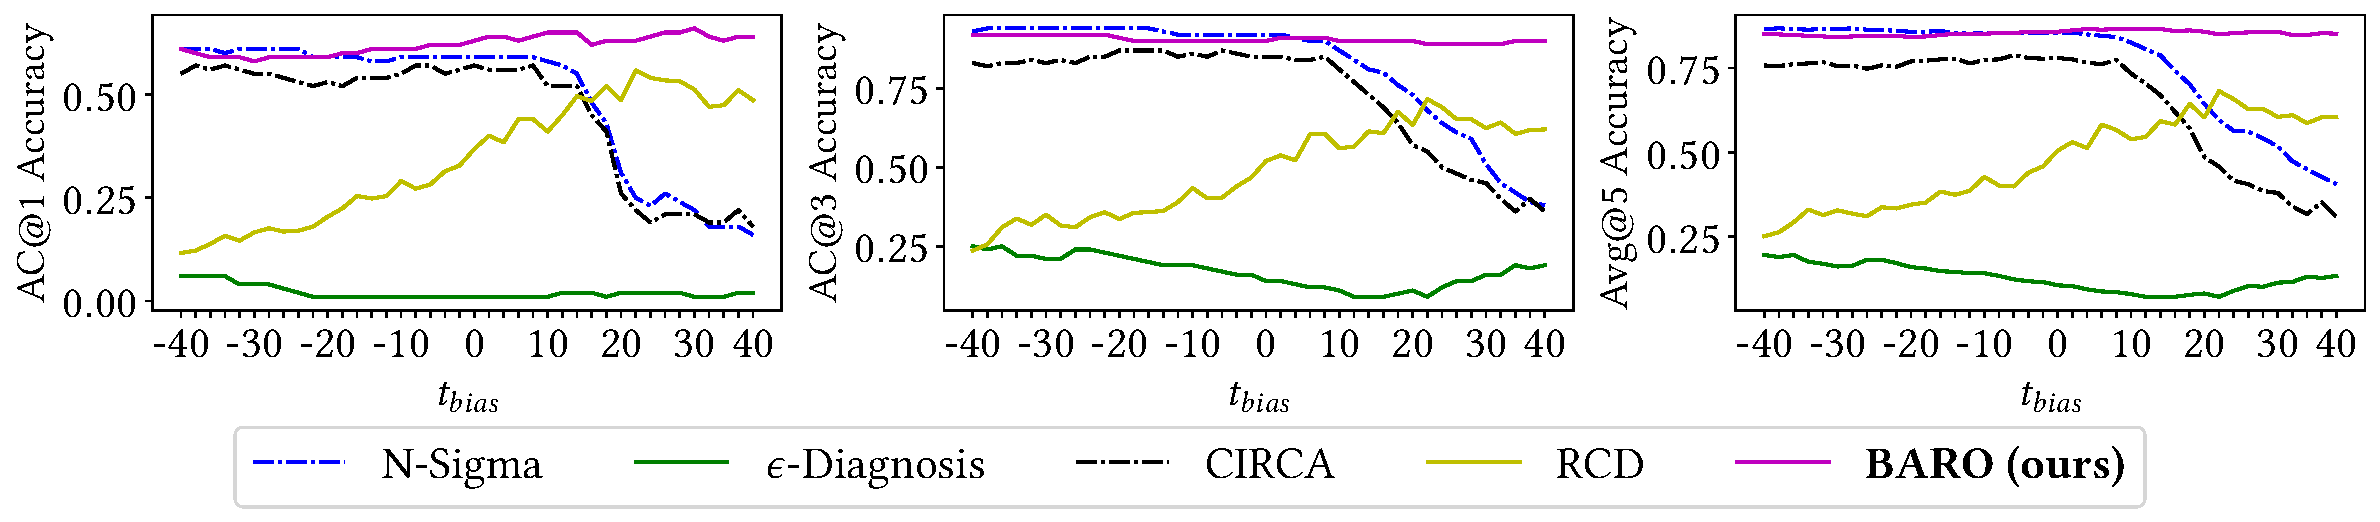
\includegraphics[width=0.9\textwidth]{image/q4-sensitivity-fse-ob-tf.pdf}
\vspace{-0.3cm}
\caption{The performance of N-Sigma, $\epsilon$-Diagnosis, CIRCA, RCD, and BARO w.r.t. different values of $t_{\text{bias}}$ on the Online Boutique dataset. The figure presents the AC@1, AC@3, and Avg@5 scores from left to right.} \label{fig:q4-sensitivity}
\vspace{-0.3cm}
\end{figure}



\subsubsection{Hyperparameter Sensitivity}

In this section, we aim to assess the sensitivity of different RCA methods to their parameters. RCD employs a divide-and-conquer strategy, requiring the specification of a chunk size parameter denoted as $\gamma$. We vary this parameter from 1 to 10 while the default value is 5. CIRCA uses PC to construct the causal graph, requiring a threshold $\alpha$ for independence testing. We vary this parameter from 0.01 to 0.5 while the default value is 0.05. $\epsilon$-Diagnosis also requires a threshold $\alpha$ to drop the insignificant metrics. We range $\alpha$ from 0.01 to 0.5 in this case.
Note that CausalRCA's parameters are already tuned \cite{Xin2023CausalRCA}, eliminating parameter sensitivities.
Fig. \ref{fig:q4-sensitivity-combine} presents our experimental results on the Online Boutique dataset whilst the experimental results on the Sock Shop dataset are in the supplementary material, Fig. S2 \cite{barogithub, barogithubzenodo}. 


% In this section, we aim to assess the sensitivity of different RCA methods to their respective parameters. RCD employs a divide-and-conquer strategy, requiring the specification of a chunk size parameter denoted as $\gamma$. We vary this parameter from 1 to 10 while the default value is 5. CIRCA uses the PC algorithm to construct the causal graph, requiring a threshold $\alpha$ for independence testing. We vary this parameter within the range of 0.01 to 0.5 while the default value is 0.05. $\epsilon$-Diagnosis also requires a threshold $\alpha$ to drop the insignificant metrics. We range $\alpha$ from 0.01 to 0.5 in this case. Note that according to \cite{Xin2023CausalRCA}, CausalRCA's parameters are already tuned, and we employ their best configuration, eliminating the need for parameter sensitivity analysis in this case. Fig. \ref{fig:q4-sensitivity-combine} presents our experimental results on the Online Boutique dataset whilst the experimental results on the Sock Shop dataset are in the supplementary material (Fig. S2) \cite{barogithub, barogithubzenodo}. 



Based on these results, it is evident that RCD, CIRCA, and $\epsilon$-Diagnosis exhibit minimal sensitivity to their parameters. Consequently, we can have confidence in the reliability of the results obtained in our %previous 
research questions. Notably, the performance of $\epsilon$-Diagnosis is identical with different values of $\alpha$. This can be attributed to the fact that in $\epsilon$-Diagnosis, the $\alpha$ parameter primarily influences the trimming of lower-ranked root causes. Given our focus on the top-k results, the length of the list becomes less critical. Similarly, for CIRCA, the main component that serves root cause analysis is its statistical scorer; the significance level $\alpha$ mainly affects the construction of the causal graph, which has minimal impact on the performance. For RCD, slight fluctuations in performance are observed with varying chunk size $\gamma$, but these variations are deemed insignificant.


\begin{figure}
\vspace{-0.2cm}
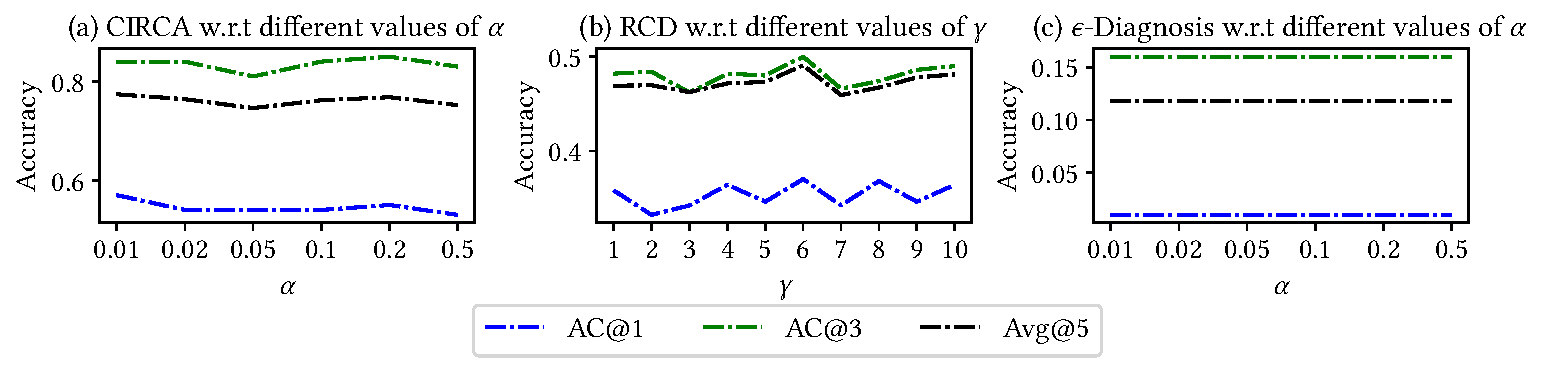
\includegraphics[width=0.95\textwidth]{image/q4-sensitivity-fse-ob-param.pdf}
\vspace{-0.2cm}
\caption{The performance of CIRCA (a), RCD (b), and $\epsilon$-Diagnosis (c) w.r.t. their different parameter values on the Online Boutique dataset. The figure presents their AC@1, AC@3, and Avg@5 scores.} \label{fig:q4-sensitivity-combine}
\vspace{-0.2cm}
\end{figure}



\subsection{Running Time \& Instrumentation Cost}

% Due to space limit, the running time analysis of different anomaly detection and RCA methods are available in our replication package \cite{barogithub}. Adopting BARO in practice necessitates the installation of monitoring agents alongside application services to gather system and application metrics. Further information on installation and how to use BARO can be found in our replication package \cite{barogithub}.


\subsubsection{Running Time}

On three datasets, BARO takes an average of 30 to 173 seconds to perform anomaly detection and root cause analysis. The highest recorded running time of BARO is 7 minutes in a case of the Train Ticket dataset. RobustScorer is very fast when it takes around 0.01 seconds to analyze the root cause, i.e., at least 3 to 1000 times faster than other methods like $\epsilon$-Diagnosis, RCD, CIRCA, and CausalRCA. The detailed running time of our proposed method and different anomaly detection and root cause analysis modules are shown in Tables \ref{tab:running-time-ad} and \ref{tab:running-time-rca}, respectively.


\begin{table}[ht]
\centering
\begin{minipage}[t]{0.48\textwidth}
\centering
\caption{Average anomaly detection run time (in seconds)}
\vspace{-0.3cm}
\label{tab:running-time-ad}
\resizebox{\textwidth}{!}{%
\begin{tabular}{l|r|r|r}
\hline
Method & \multicolumn{1}{c|}{\textbf{Online Boutique}} & \multicolumn{1}{c|}{\textbf{Sock Shop}} & \multicolumn{1}{c}{\textbf{Train Ticket}} \\ \hline \hline
N-Sigma & 0.16 & 0.11 & 0.53 \\ \hline
BIRCH & 0.05 & 0.04 & 0.11 \\ \hline
SPOT & 3.17 & 1.9 & 11.4 \\ \hline
UniBCD & 819.7 & 638.19 & 3292.48 \\ \hline
\textbf{BARO (Ours)} & 44.83 & 30 & 173.37 \\ \hline
\end{tabular}%
}

% {\footnotesize \textit{(*) Univariate Bayesian Online Change Point Detection.}}
\end{minipage}
\hfill
\begin{minipage}[t]{0.48\textwidth}
\centering
\caption{Average RCA run time (in seconds)}
\vspace{-0.2cm}
\label{tab:running-time-rca}
\resizebox{\textwidth}{!}{%
\begin{tabular}{l|r|r|r}
\hline
Method & \multicolumn{1}{l|}{\textbf{Online Boutique}} & \multicolumn{1}{l|}{\textbf{Sock Shop}} & \multicolumn{1}{l}{\textbf{Train Ticket}} \\ \hline \hline 
CausalRCA & 299.18 & 287.18 & 2638.51 \\ \hline
$\epsilon$-Diagnosis & 3.94 & 3.97 & 14.83 \\ \hline
RCD & 10.74 & 5.62 & 24.21 \\ \hline
CIRCA & 13.52 & 13.47 & 7564.88 \\ \hline
N-Sigma & 0.01 & 0.01 & 0.01 \\ \hline
\textbf{BARO (Ours)} & 0.01 & 0.01 & 0.01 \\ \hline
\end{tabular}%
}
\end{minipage}
\vspace{-0.3cm}
\end{table}


\subsubsection{Instrumentation Cost}

BARO requires monitoring agents (e.g., Istio, cAdvisor, Prometheus) installed alongside application services to collect system-level (e.g., CPU/Mem/Disk usage) and application-level metrics (e.g., response time, request count per minute). These metrics are used for BARO to perform anomaly detection and root cause analysis. BARO requires Python and some standard packages (e.g. pandas, numpy). Further details are available in our artifacts \cite{barogithub, barogithubzenodo}.
